\documentclass{bmstu}[a4paper]

\renewcommand\labelitemi{---}
\setenumerate[0]{label=\arabic*)}

\usepackage{threeparttable}

\bibliography{biblio}

\begin{document}

\makereporttitle
{Информатика и системы управления} % Название факультета
{Программное обеспечение ЭВМ и информационные технологии} % Название кафедры
{лабораторной работе №~2} % Название работы (в дат. падеже)
{Анализ алгоритмов} % Название курса (необязательный аргумент)
{Умножение матриц} % Тема работы
{} % Номер варианта (необязательный аргумент)
{Писаренко~Д.~П./ИУ7-54Б} % Номер группы/ФИО студента (если авторов несколько, их необходимо разделить запятой)
{Волкова~Л.~Л.} % ФИО преподавателя

\maketableofcontents

\chapter*{ВВЕДЕНИЕ}
\addcontentsline{toc}{chapter}{ВВЕДЕНИЕ}

Сортировка данных является фундаментальной задачей в области информатики и алгоритмов. 
Независимо от конкретной области применения, эффективные алгоритмы сортировки существенно влияют на производительность программных систем. 
От правильного выбора алгоритма зависит как время выполнения программы, так и затраты ресурсов компьютера \cite{knut}.

Алгоритмы сортировки находят применение в следующих сферах:
\begin{itemize}
	\item базы данных;
	\item анализ данных и статистика;
	\item алгоритмы машинного обучения;
	\item криптография.
\end{itemize}

Цель данной лабораторной работы --- рассмотреть алгоритмы сортировки.
Для достижения поставленной цели необходимо выполнить следующие задачи:
\begin{itemize}
	\item описать алгоритмы блочной, быстрой сортировок и сортировку выбором;
	\item разработать программное обеспечение, реализующее алгоритмы сортировок;
	\item выбрать инструменты для реализации и замера процессорного времени
	выполнения реализаций алгоритмов;
	\item проанализировать затраты реализаций алгоритмов по времени.
\end{itemize}

\chapter{Аналитический раздел}

Матрицей называется прямоугольная таблица чисел, вида \eqref{eq:matrix}, состоящая из $m$ строк и $n$ столбцов \cite{matrix}.

\begin{equation}
	\label{eq:matrix}
	\begin{pmatrix}
		a_{11} & a_{12} & \ldots & a_{1n}\\
		a_{21} & a_{22} & \ldots & a_{2n}\\
		\vdots & \vdots & \ddots & \vdots\\
		a_{m1} & a_{m2} & \ldots & a_{mn}
	\end{pmatrix},
\end{equation}

Пусть $A$ --- матрица, тогда $а_{ij}$ --- элемент этой матрицы, который находится на \textit{i-ой} строке и \textit{j-ом} столбце.

Если количество столбцов первой матрицы совпадает с количеством строк второй матрицы, то возможно выполнить их матричное умножение.
В результате умножения получится матрица-произведение, количество строк в которой равно количеству строк первой матрицы, а количество столбцов равно количеству столбцов второй матрицы.

\section{Классический алгоритм}

Пусть даны две прямоугольные матрицы $A$ и $B$ размеров $[m \times n]$ и $[n \times k]$ соответственно. В результате произведение матриц $A$ и $B$ получим матрицу $C$ размера $[m \times k]$, элементы которой вычисляются по \eqref{eq:matrix_classic}.

\begin{equation}
	\label{eq:matrix_classic}
	c_{ij} = \sum_{l=1}^{n}a_{il}b_{lj}
\end{equation}

Классический алгоритм умножения матриц, реализует формулу \eqref{eq:matrix_classic}.

\section{Алгоритм Винограда}

Произведение матриц $A$ и $B$ можно связать со скалярным  произведением строки матрицы $A$ на столбец матрицы $B$ \cite{book_vinograd}.

Рассмотрим два вектора $V = (v1, v2, v3, v4)$ и $W = (w1, w2, w3, w4)$.  

Их скалярное произведение равно (\ref{formula}).

\begin{equation} \label{formula}
	V \cdot W=v_1 \cdot w_1 + v_2 \cdot w_2 + v_3 \cdot w_3 + v_4 \cdot w_4
\end{equation}

Равенство (\ref{formula}) можно переписать в виде (\ref{formula2}) 
\begin{equation} \label{formula2}
	V \cdot W=(v_1 + w_2) \cdot (v_2 + w_1) + (v_3 + w_4) \cdot (v_4 + w_3) - v_1 \cdot v_2 - v_3 \cdot v_4 - w_1 \cdot w_2 - w_3 \cdot w_4
\end{equation}

Теперь допустим, что у нас есть две матрицы $A$ и $B$ размерности $m \times n$ и $n \times p$ соответственно, и мы хотим найти их произведение $C = A \cdot B$.
Тогда алгоритм будет состоять из следующих шагов.

\begin{enumerate}
	\item Подготовительные вычисления. Сначала создаются два вспомогательных массива \eqref{eq:rf} и \eqref{eq:cf}.
	\begin{equation}
	\label{eq:rf}
	\text{{rowFactor}}[i] = \sum_{j=0}^{n/2 - 1} A[i][2j+1] \cdot A[i][2j]
	\end{equation}
	для \(0 \leq i < m\)
	\begin{equation}
	\label{eq:cf}
	\text{{colFactor}}[j] = \sum_{i=0}^{n/2 - 1} B[2i+1][j] \cdot B[2i][j]
	\end{equation}
	для \(0 \leq j < p\).
	
	\item Умножение матриц. Вычисляем результирующую матрицу $C$ по формуле~\eqref{eq:c_res}.
	\begin{equation}
		\label{eq:c_res}
		\begin{aligned}
			C[i][j] &= \sum_{k=0}^{n/2 - 1} (A[i][2k+1] + B[2k][j]) \cdot (A[i][2k] + B[2k+1][j]) \\
			&\quad - \text{{rowFactor}}[i] - \text{{colFactor}}[j]
		\end{aligned}
	\end{equation}
	для \(0 \leq i < m\) и \(0 \leq j < p\).
	
	\item Коррекция. Если \(n\) нечетно, добавляем коррекцию, в соответствии с формулой \eqref{eq:er}.
	\begin{equation}
		\label{eq:er}
	C[i][j] += A[i][n] \cdot B[n][j]
	\end{equation}
	для \(0 \leq i < m\) и \(0 \leq j < p\). 
\end{enumerate}

\section{Алгоритм Штрассена}

Алгоритм Штрассена --- это алгоритм умножения квадратных матриц, который является более эффективным для больших матриц, чем классический метод умножения \cite{strassen}.

Если добавить к матрицам $A$ и $B$ одинаковые нулевые строки и столбцы, их произведение станет равно матрице $C$ с теми же добавленными строками и столбцами. 
Поэтому в данном алгоритме рассматриваются матрицы порядка $2^{k + 1}$, где $ k \in \mathbb{N} $, а все остальные матрицы, сводятся к этому размеру добавлением нулевых строк и столбцов. 

Алгоритм состоит из следующих шагов.

\begin{enumerate}
	\item Разбиение матриц \eqref{eq:mat_split}.
	\begin{equation}
		\label{eq:mat_split}
	A = \begin{bmatrix} A_{11} & A_{12} \\ A_{21} & A_{22} \end{bmatrix}, \quad
	B = \begin{bmatrix} B_{11} & B_{12} \\ B_{21} & B_{22} \end{bmatrix}
	,
	\end{equation} где $A_{ij}$ и $B_{ij}$ -- матрицы порядка $2^{k}$
	
	\item Вычисление вспомогательных матриц \eqref{eq:help_mat}.
	\begin{equation}
		\label{eq:help_mat}
	\begin{aligned}
		M_1 &= (A_{11} + A_{22})(B_{11} + B_{22}) \\
		M_2 &= (A_{21} + A_{22})B_{11} \\
		M_3 &= A_{11}(B_{12} - B_{22}) \\
		M_4 &= A_{22}(B_{21} - B_{11}) \\
		M_5 &= (A_{11} + A_{12})B_{22} \\
		M_6 &= (A_{21} - A_{11})(B_{11} + B_{12}) \\
		M_7 &= (A_{12} - A_{22})(B_{21} + B_{22})
	\end{aligned}
	\end{equation}
	
	\item Вычисление результирующих подматриц \eqref{eq:res_submat}.
	\begin{equation}
		\label{eq:res_submat}
	\begin{aligned}
		C_{11} &= M_1 + M_4 - M_5 + M_7 \\
		C_{12} &= M_3 + M_5 \\
		C_{21} &= M_2 + M_4 \\
		C_{22} &= M_1 - M_2 + M_3 + M_6
	\end{aligned}
	\end{equation}
		
	Результирующая матрица состоит из $C_{ij}$~\eqref{eq:res_mat_str}.
	\begin{equation}
		\label{eq:res_mat_str}
		AB = C = \begin{bmatrix} C_{11} & C_{12} \\ C_{21} & C_{22} \end{bmatrix}
	\end{equation}
		
\end{enumerate}


\section*{Вывод}
В данном разделе были описаны алгоритмы классического умножения матриц, алгоритм Штрассена и алгоритм Винограда.
\chapter{Конструкторский раздел}

В этом разделе будет представлено описание используемых типов данных, а также схематические изображения алгоритмов сортировок: блочной, быстрой и выбором.

\section{Требования к программному обеспечению}

Программа должна поддерживать два режима работы: режим массового замера времени и режим сортировки введенного массива.

Режим массового замера времени должен обладать следующей функциональностью:
\begin{itemize}
	\item генерировать массивы различного размер для проведения замеров;
	\item осуществлять массовый замер, используя сгенерированные данные;
	\item результаты массового замера должны быть представлены в виде таблицы и графика.
\end{itemize}

К режиму сортировки выдвигается следующий ряд требований:
\begin{itemize}
	\item возможность работать с массивами разного размера, которые вводит пользователь;
	\item наличие интерфейса для выбора действий;
	\item на выходе программы массив, отсортированный тремя алгоритмами по возрастанию.
\end{itemize}

\section{Описание используемых типов данных}

При реализации алгоритмов будут использованы следующие структуры и типы данных:
\begin{itemize}
	\item целое число представляет количество элементов в массиве;
	\item список целых чисел;
\end{itemize}

\section{Разработка алгоритмов}

На рисунке \ref{pic:blocksort} приведена схема алгоритма блочной сортировки.

\begin{figure}[H]
	\centering
	
\includegraphics[scale=0.62]{assets/blocksort.pdf}
	\caption{Схема алгоритма блочной сортировки}
	\label{pic:blocksort}
\end{figure}

\newpage

На рисунке \ref{pic:quicksort} приведена схема алгоритма быстрой сортировки.

\begin{figure}[H]
	\centering
	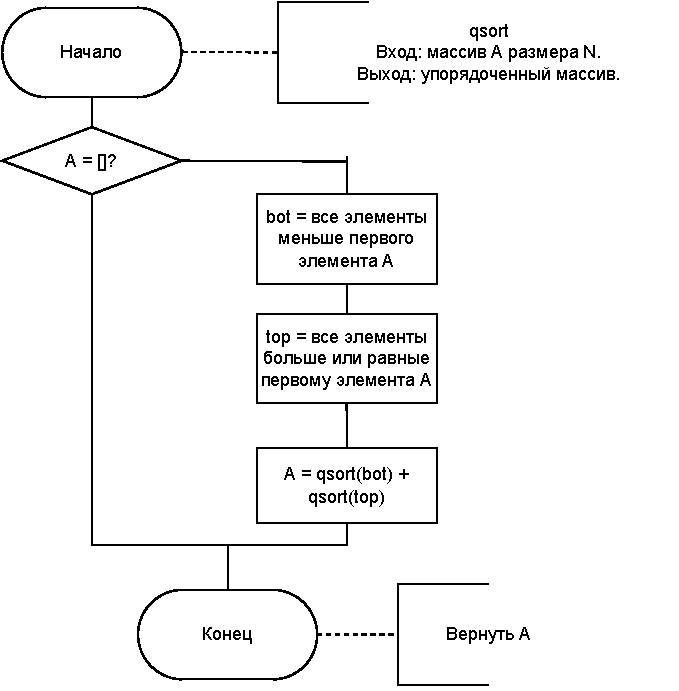
\includegraphics[scale=0.62]{assets/quicksort.pdf}
	\caption{Схема алгоритма быстрой сортировки}
	\label{pic:quicksort}
\end{figure}

\newpage

На рисунке \ref{pic:selectionsort} приведена схема алгоритма сортировки выбором.

\begin{figure}[H]
	\centering
	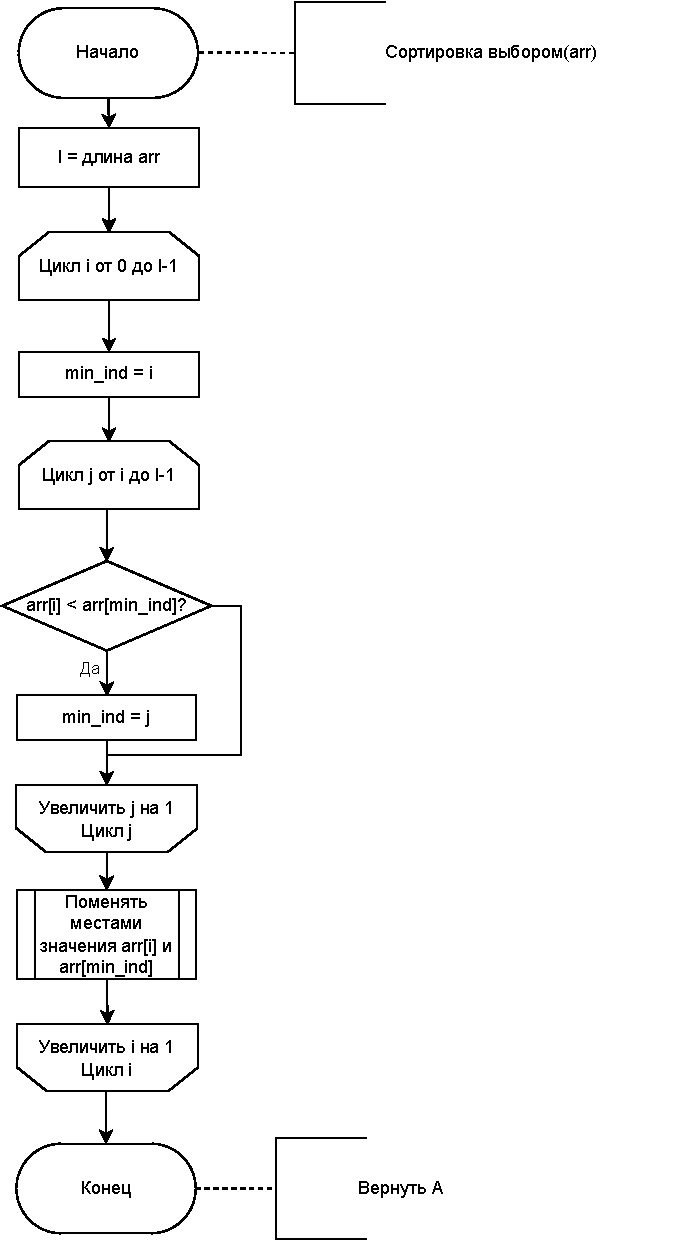
\includegraphics[scale=0.62]{assets/selectionsort.pdf}
	\caption{Схема алгоритма сортировки выбором}
	\label{pic:selectionsort}
\end{figure}

\newpage


\section{Оценка трудоемкости алгоритмов}

Модель для оценки трудоемкости алгоритмов состоит из шести пунктов:
\begin{enumerate}
	\item $+, -, =, +=, -=, ==, ||, \&\&, <, >, <=, >=, <<, >>, []$ --- считается, что эти операции обладают трудоемкостью в 1 единицу;
	\item $*, /, *=, /=, \% $ --- считается, что эти операции обладают трудоемкостью в 2 единицы;
	\item трудоемкость условного перехода принимается за $0$;
	\item трудоемкость условного оператора рассчитывается по формуле \eqref{eq:if},
	\begin{equation}
		\label{eq:if}
		f_{if} = f_{\text{условия}} + 
		\begin{cases}
			min(f_1, f_2), & \text{лучший случай}\\
			max(f_1, f_2), & \text{худший случай}
		\end{cases},
	\end{equation}
	где $f_1$ --- трудоемкость блока, который вычисляется при выполнении условия, а $f_2$ --- трудоемкость блока, который вычисляется при невыполнении условия;
	\item трудоемкость цикла рассчитывается по формуле \eqref{eq:for},
	\begin{equation}
		\label{eq:for}
		\begin{gathered}
			f_{for} = f_{\text{инициализация}} + f_{\text{сравнения}} + M_{\text{итераций}} \cdot (f_{\text{тело}} +\\
			+ f_{\text{инкремент}} + f_{\text{сравнения}});
		\end{gathered}
	\end{equation}
	\item вызов подпрограмм и передача параметров принимается за $0$.
\end{enumerate}

\subsection{Трудоемкость алгоритма блочной сортировки}

В данной реализации размер блока обозначается как $k$, трудоемкость операции добавления и удаления элемента из вектора равна 2.


\textbf{Лучший случай:} массив отсортирован, элементы распределены равномерно (все блоки содержат одинаковое число элементов), расчет трудоемкости данного случая приведен в (\ref{сomplexity:block_best}).


\begin{equation}
	\label{сomplexity:block_best}
	\begin{gathered}
		f_{best} = 1 +1 + \frac{n}{k} \cdot(1 + 2+f_{shaker} + 2 + 1 + 4 + \\
		+ k \cdot (3 + 1 + 4)) + 1 + 1 + \\
		+ \frac{n}{k} \cdot (1 + 4 + 1 + 1 + 5 + 1 + 4 + 1 + 1 + n \cdot (5)) = \\
		= 4 + \frac{29\cdot n + n \cdot f_{shaker} + 5 \cdot n^2}{k}  + 8 \cdot n  = \\
		= 4 + 8 \cdot n + 29 \cdot \frac{n}{k} + n \cdot (14.5 + \frac{k}{2}) + \frac{5 \cdot n^2}{k}.
	\end{gathered}
\end{equation}

\textbf{Худший случай:} большое количество пустых блоков, массив отсортирован в обратном порядке (худший случай сортировки перемешиванием, которая используется в блочной сортировке), расчет трудоемкости приведен в выражении (\ref{сomplexity:block_worst}).

\begin{equation}
	\label{сomplexity:block_worst}
	\begin{gathered}
		f_{worst} = 1 +1 + \frac{n}{k} \cdot(1 + 2+f_{shaker} + 2 + 1 + 4 + \\
		+ k \cdot (3 + 1 + 4)) + 1 + 1 + \\
		 + \frac{n}{k} \cdot (1 + 4 + 1 + 1 + 5 + 1 + 4 + 1 + 1 + k \cdot (6)) = \\
		= 4 + \frac{29\cdot n + n \cdot f_{shaker} + 6 \cdot n^2}{k}  + 8 \cdot n  = \\
		= 4 + 8 \cdot n + 29 \cdot \frac{n}{k} + n \cdot (19.5 + \frac{k}{2}) + \frac{6 \cdot n^2}{k}.
	\end{gathered}
\end{equation}


\textbf{Вывод о трудоемкости блочной сортировки}

Данная реализация зависит от выбранного размера блока, а также от количества сортируемых элементов. В соответствии с выражениями (\ref{сomplexity:block_worst} , \ref{сomplexity:block_best})  операнды $\frac{n \cdot k}{2}$, $\frac{n^2}{k}$ и $\frac{n}{k}$ зависят от значений $n$ и $k$, первый приведенный операнд возрастает при увеличении $k$, другие убывают.


\subsection{Трудоемкость алгоритма гномьей сортировки}

Для данной сортировки лучшим случаем является отсортированный массив, тогда трудоемкость алгоритма будет рассчитываться по формуле \eqref{eq:gnome_best}.
\begin{equation}
	\label{eq:gnome_best}
	\begin{gathered}
		f_{best} = 1 + 1 + (N - 1)(1 + 1 + 4 + 1) = 7 N - 5 \approx O(N)
	\end{gathered}
\end{equation}

Для данного алгоритма худшим является случай, когда массив отсортирован в обратном порядке, тогда трудоемкость рассчитывается по \eqref{eq:gnome_worst}.
\begin{equation}
	\label{eq:gnome_worst}
	\begin{gathered}
		f_{worst} = 1 + 1 + \frac{(N + 1)N}{2}(1 + 1 + 4 + 9 + 1) + N + \\
		+ \frac{(N + 1)N}{2}(1 + 1 + 4 + 1) = 
		\\ = \frac{23}{2} N^2 + \frac{25}{2}N + 2 \approx O(N^2)
	\end{gathered}
\end{equation}

\subsection{Трудоемкость алгоритма сортировки выбором}

Трудоемкость сортировки выбором в худшем случае $(O(N^2)$
Трудоемкость сортировки выбором в лучшем случае $(O(N^2))$


\section*{Вывод}
На основе теоретических данных, полученных из аналитического раздела были построены схемы требуемых алгоритмов. 
Была введена модель оценки трудоемкости алгоритма, были рассчитаны трудоемкости алгоритмов в соответствии с этой моделью.

В результате теоретической оценки трудоемкостей алгоритмов выяснилось, что лучшей асимптотической оценкой в худшем случае обладает пирамидальная сортировка $O(N \log_{2}N)$. 
Алгоритм гномьей сортировки оказывается лучше всех прочих сортировок в лучшем случае (т.~е. для отсортированных массивов), обладая асимптотической сложностью $O(N)$, но при худшем случае проигрывает по константе алгоритму Шелла, т.~о. асимптотическая сложность в худшем случае у гномьей сортировки $O(\frac{23}{2}N^2)$, а у Шелла $O(\frac{32}{3} N ^ 2)$. 
В лучшем случае асимптотическая сложность алгоритма Шелла $O(10N\log_2N)$ меньше, чем асимптотическая сложность алгоритма пирамидальной сортировки $O(29N\log_2N)$.
\chapter{Технологический раздел}

В данном разделе будут приведены требования к программному обеспечению, средства реализации, листинг кода и функциональные тесты.

\section{Средства реализации}

Для реализации данной работы был выбран язык \textit{Python}~\cite{python}.
Данный выбор обусловлен следующим:
\begin{itemize}
	\item язык поддерживает все структуры данных, которые выбраны в результате проектирования;
	\item язык позволяет реализовать все алгоритмы, выбранные в результате проектирования;
	\item язык позволяет замерять процессорное время с помощью модуля \textit{time}. 
\end{itemize}

Процессорное время было замерено с помощью функции \textit{process\_time()} из модуля \textit{time}~\cite{python-time}.

\section{Сведения о модулях программы}

Данная программа разбита на следующие модули:
\begin{itemize}
	\item $main.py$ --- файл, содержащий функцию $main$;
	\item $functions.py$ --- файл, содержащий вспомогательные функции (ввод массива с клавиатуры, рандомно, с файла и т.д.)
	\item $sorts.py$ --- файл, содержащий код реализаций всех алгоритмов сортировок;
	\item $tests.py$ --- файл, в котором содержатся функции для замера и вывода времени выполнения реализаций алгоритмов.
\end{itemize}

\section{Реализация алгоритмов}

\clearpage

\section{Функциональные тесты}

В таблице \ref{tbl:func_tests} приведены функциональные тесты для разработанных алгоритмов сортировок. Все тесты пройдены успешно.

\begin{table}[ht]
	\small
	\begin{center}
		\begin{threeparttable}
			\caption{Функциональные тесты}
			\label{tbl:func_tests}
			\begin{tabular}{|c|c|c|}
				\hline
				\bfseries Массив
				& \bfseries Ожидаемый результат
				& \bfseries Фактический результат \\ 
				\hline
				[1, 2, 3, 4, 5] & [1, 2, 3, 4, 5] & [1, 2, 3, 4, 5] \\
				\hline
				[5, 4, 3, 2, 1]  & [1, 2, 3, 4, 5] & [1, 2, 3, 4, 5] \\
				\hline
				[~]  & [~] & [~] \\
				\hline
				[1]  & [1] & [1]\\
				\hline
				[4, 1, 2, 3]  & [1, 2, 3, 4] & [1, 2, 3, 4] \\
				\hline
				[2, 1]  & [1, 2] & [1, 2] \\
				\hline
				[31, 57, 24, -10, 59]  & [-10, 24, 31, 57, 59] & [-10, 24, 31, 57, 59] \\
				\hline
			\end{tabular}	
		\end{threeparttable}	
	\end{center}
\end{table}


\section*{Вывод}
Были разработаны и протестированы спроектированные алгоритмы сортировок: блочная, быстрая и выбором.
\chapter{Исследовательский раздел}

В данном разделе будут приведены: пример работы программы, постановка эксперимента и сравнительный анализ алгоритмов на основе полученных данных.

\section{Демонстрация работы программы}


На рисунке \ref{img:program} представлена демонстрация работы разработанного программного обеспечения, а именно показаны результаты сортировки массива $[3, 5, -3, 1, 2, 4, -6, 2]$.

\includeimage
{program} % Имя файла без расширения (файл должен быть расположен в директории inc/img/)
{f} % Обтекание (без обтекания)
{h} % Положение рисунка (см. figure из пакета float)
{0.65\textwidth} % Ширина рисунка
{Демонстрация работы программы при сортировке массива} % Подпись рисунка

\clearpage


\section{Технические характеристики}

Технические характеристики компьютера, на котором проводился замерный эксперимент:
\begin{itemize}
	\item процессор Intel Core i5-10400F (6 ядер) \cite{intel};
	\item 16 Гб оперативная память DDR4;
	\item операционная система Windows 10 Pro \cite{windows}.
\end{itemize}

Во время проведения исследования компьютер был нагружен только системными приложениями и целевой программой.

\section{Время выполнения реализаций алгоритмов}

Результаты замеров времени выполнения реализаций алгоритмов сортировок приведены в таблицах \ref{tbl:time_measurements} -- \ref{tbl:time_measurements_rand}.
Замеры времени проводились на массивах одного размера и усреднялись для каждого набора одинаковых экспериментов.

В таблицах \ref{tbl:time_measurements} -- \ref{tbl:time_measurements_rand} используются следующие обозначения: 
\begin{itemize}
	\item Блочная --- реализация алгоритма блочной сортировки;
	\item Быстрая --- реализация алгоритма быстрой сортировки;
	\item Выбором --- реализация алгоритма сортировки выбором.
\end{itemize}

\begin{table}[h]
	\begin{center}
		\begin{threeparttable}
			\captionsetup{justification=raggedright,singlelinecheck=off}
			\caption{Время работы реализации алгоритмов на неотсортированных массивах (в мс)}
			\label{tbl:time_measurements}
			\begin{tabular}{|c|c|c|c|}
				\hline
				Размер массива & Блочная & Быстрая & Выбором \\
				\hline
				100 &$ 0.078125 $&$ 0.125 $&$ 0.203125 $\\
				\hline
				200 &$ 0.203125 $&$ 0.265625 $&$ 0.90625 $\\
				\hline
				300 &$ 0.40625 $&$ 0.5 $&$ 1.78125 $\\
				\hline
				400 &$ 0.765625 $&$ 0.546875 $&$ 3.484375 $\\
				\hline
				500 &$ 1.078125 $&$ 0.734375 $&$ 5.625 $\\
				\hline
				600 &$ 1.390625 $&$ 0.890625 $&$ 7.8125 $\\
				\hline
				700 &$ 1.8125 $&$ 1.15625 $&$ 10.609375 $\\
				\hline
				800 &$ 2.234375 $&$ 1.25 $&$ 14.25 $\\
				\hline
				900 &$ 2.984375 $&$ 1.296875 $&$ 18.0625 $\\
				\hline
				1000 &$ 3.734375 $&$ 1.5 $&$ 22.515625 $\\
				\hline
			\end{tabular}
		\end{threeparttable}
	\end{center}
\end{table}

\begin{table}[h]
	\begin{center}
		\begin{threeparttable}
			\captionsetup{justification=raggedright,singlelinecheck=off}
			\caption{Время работы реализации алгоритмов на отсортированных в обратном порядке массивах (в мс)}
			\label{tbl:time_measurements_sorted}
			\begin{tabular}{|c|c|c|c|}
				\hline
				Размер массива & Блочная & Быстрая & Выбором \\
				\hline
				100 &$ 0.078125 $&$ 0.125 $&$ 0.203125 $\\
				\hline
				200 &$ 0.203125 $&$ 0.25 $&$ 0.765625 $\\
				\hline
				300 &$ 0.40625 $&$ 0.390625 $&$ 1.9375 $\\
				\hline
				400 &$ 0.640625 $&$ 0.546875 $&$ 3.3475 $\\
				\hline
				500 &$ 0.96875 $&$ 0.6875 $&$ 5.375 $\\
				\hline
				600 &$ 1.328125 $&$ 0.875 $&$ 7.609375 $\\
				\hline
				700 &$ 1.75 $&$ 1.046875 $&$ 10.640625 $\\
				\hline
				800 &$ 2.609375 $&$ 1.140625 $&$ 14.046875 $\\
				\hline
				900 &$ 2.9375 $&$ 1.25 $&$ 17.828125 $\\
				\hline
				1000 &$ 3.71875 $&$ 1.4375 $&$ 22.265625 $\\
				\hline
			\end{tabular}
		\end{threeparttable}
	\end{center}
\end{table}

\begin{table}[h]
	\begin{center}
		\begin{threeparttable}
			\captionsetup{justification=raggedright,singlelinecheck=off}
			\caption{Время работы реализации алгоритмов на отсортированных массивах (в мс)}
			\label{tbl:time_measurements_rand}
			\begin{tabular}{|c|c|c|c|}
				\hline
				Размер массива & Блочная & Быстрая & Выбором \\
				\hline
				100 &$ 0.0625 $&$ 0.109375 $&$ 0.203125 $\\
				\hline
				200 &$ 0.203125 $&$ 0.3125 $&$ 0.828125 $\\
				\hline
				300 &$ 0.390625 $&$ 0.4375 $&$ 1.859375 $\\
				\hline
				400 &$ 0.640625 $&$ 0.578125 $&$ 3.453125 $\\
				\hline
				500 &$ 1 $&$ 0.6875 $&$ 5.3125 $\\
				\hline
				600 &$ 1.3125 $&$ 0.859375 $&$ 7.90625 $\\
				\hline
				700 &$ 1.890625 $&$ 1.03125 $&$ 10.46875 $\\
				\hline
				800 &$ 2.28125 $&$ 1.125 $&$ 13.8125 $\\
				\hline
				900 &$ 2.9375 $&$ 1.3125 $&$ 18.109375 $\\
				\hline
				1000 &$ 3.4375 $&$ 1.4375 $&$ 22.421875 $\\
				\hline
			\end{tabular}
		\end{threeparttable}
	\end{center}
\end{table}

\clearpage
На рисунках \ref{pic:random} -- \ref{pic:sorted} изображены графики зависимостей времени выполнения реализаций сортировок от размеров массивов.

\begin{figure}[H]
	\centering
	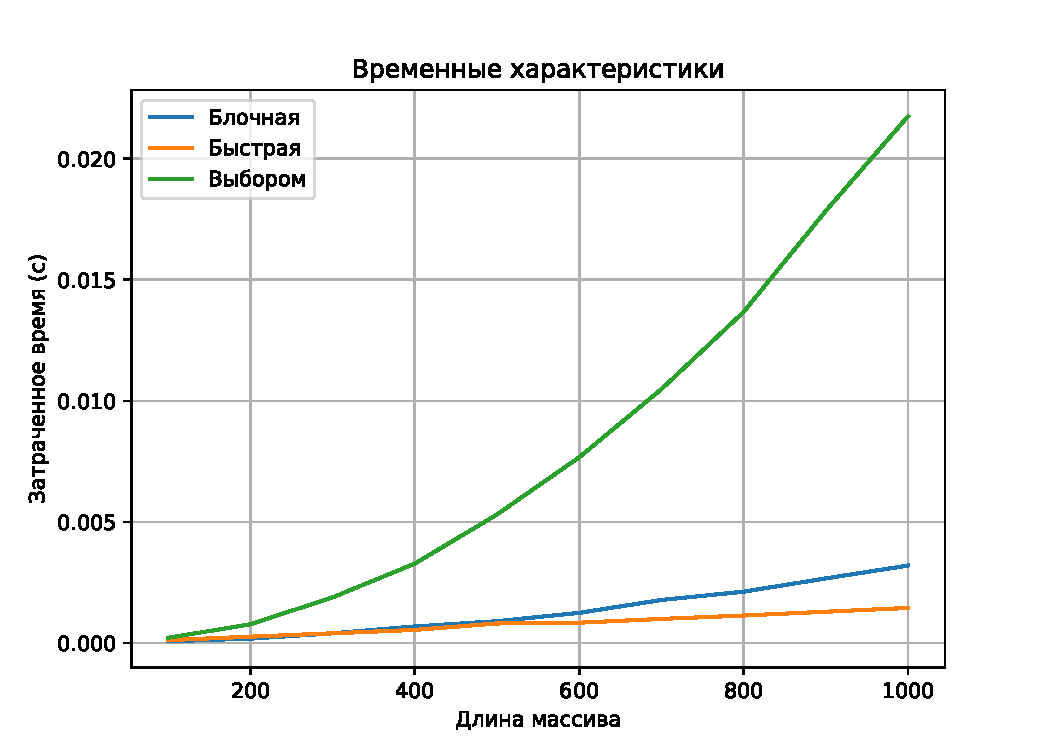
\includegraphics[scale=0.62]{assets/plots/cpu-random.pdf}
	\caption{Сравнение реализаций алгоритмов по времени выполнения на неотсортированных массивах}
	\label{pic:random}
\end{figure}

\newpage

\begin{figure}[H]
	\centering
	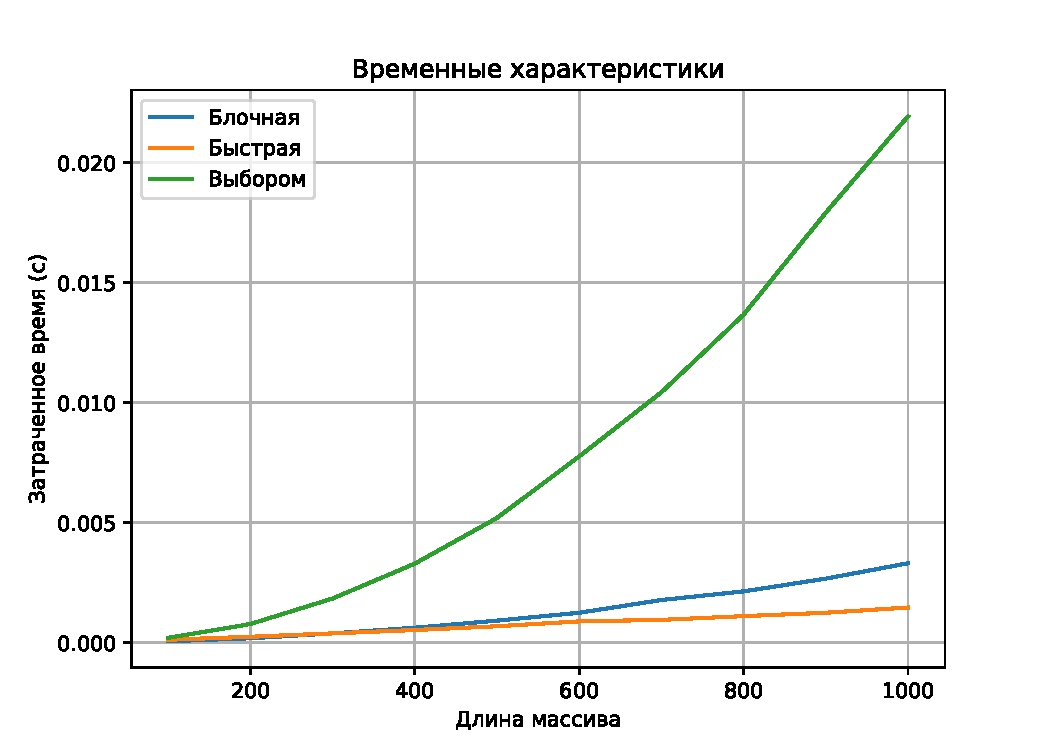
\includegraphics[scale=0.62]{assets/plots/cpu-reversed.pdf}
	\caption{Сравнение реализаций алгоритмов по времени выполнения на отсортированных в обратном порядке массивах}
	\label{pic:reversed}
\end{figure}

\newpage

\begin{figure}[H]
	\centering
	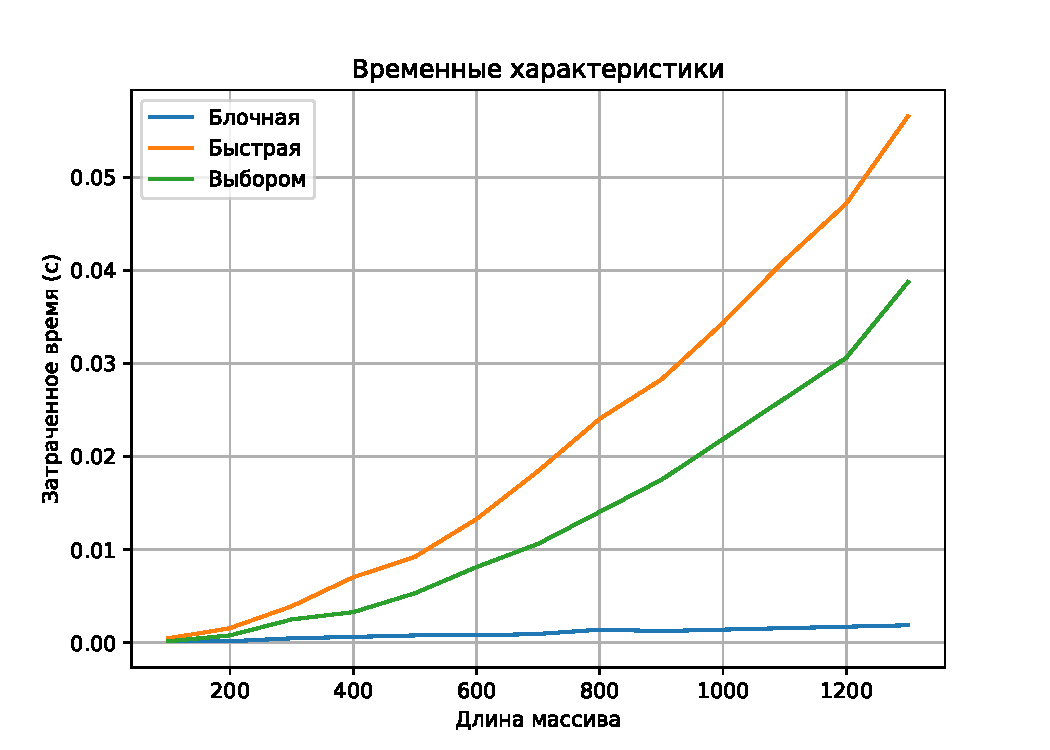
\includegraphics[scale=0.62]{assets/plots/cpu-sorted.pdf}
	\caption{Сравнение реализаций алгоритмов по времени выполнения на отсортированных массивах}
	\label{pic:sorted}
\end{figure}

\clearpage


\section*{Вывод}

В результате замеров времени выполнения реализаций различных алгоритмов было выявлено, что для массивов длины 1000, отсортированных в обратном порядке, реализация алгоритма быстрой сортировки по времени оказалась в 2.59 раз лучше, чем реализация блочной сортировки, и в 15.49 раз лучше реализации сортировки выбором. 
В свою очередь, реализация блочной сортировки оказалась лучше в 5.99 раз по времени выполнения, чем реализация  сортировки выбором.

Для отсортированных массивов длиной 1000 реализация быстрой сортировки оказалась лучше по времени в 2.39 раз, чем реализация блочной сортировки, и в 15.6 раз лучше, чем реализация сортировки выбором. 
В свою очередь, реализация блочной сортировки оказалась лучше в 6.52 раз по времени выполнения, чем реализация сортировки выбором.

Для случайно упорядоченных массивов длиной 1000 реализация быстрой сортировки оказалась лучше по времени в 2.49 раз, чем реализация блочной сортировки, и в 15.01 раза лучше, чем реализация сортировки выбором. 
В свою очередь, реализация блочной сортировки на случайно упорядоченных массивах оказалась лучше в 6.03 раза по времени выполнения, чем реализация сортировки выбором.

Стоит заметить, что для массивов длиной менее 300, реализация блочной сортировки была лучше или такой же по времени выполнения по сравнению с быстрой сортировкой, но на массивах ллины более 300 быстрая сортировка становилась лучше по времени выполнению.
\chapter*{ЗАКЛЮЧЕНИЕ}
\addcontentsline{toc}{chapter}{ЗАКЛЮЧЕНИЕ}

Цель данной лабораторной работы была достигнута, а именно были исследованы алгоритмы умножения матриц.


Для достижения поставленной цели были выполнены следующие задачи.
\begin{enumerate}
	\item Описаны следующие алгоритмы умножения матриц:
	\begin{itemize}
		\item классический алгоритм;
		\item алгоритм Винограда;
		\item алгоритм Штрассена.
	\end{itemize}
	\item Проведена оптимизация алгоритма Винограда.
	\item Разработано программное обеспечение, реализующее алгоритмы умножения.
	\item Выбраны инструменты для реализации алгоритмов и замера процессорного времени их выполнения.
	\item Проведен анализ затрат реализаций алгоритмов по времени. 
\end{enumerate}

В результате исследования реализаций алгоритмов было выявлено, что для матриц с порядком 51, реализация алгоритма Винограда оказалась в 1.02 раза хуже реализации классического алгоритма по времени выполнения, при этом реализация алгоритма Винограда с оптимизациями оказалась лучше в 1.34 раза реализации классического алгоритма и в 1.37 раз лучше реализации без оптимизаций по времени выполнения. 
Для матриц с четным порядком 46, реализация алгоритма Винограда хуже реализации классического алгоритма в 1.02 раза по времени выполнения, а реализация алгоритма Винограда с оптимизацией оказалась лучше классического алгоритма в 1.32 раза. 

Для матриц с порядком 51, реализация алгоритма Штрассена оказалась хуже по времени выполнения в 5.24 раза, в 5.14 раза и в 7.04 раза, чем реализации классического алгоритма, алгоритма Винограда и алгоритма Винограда с оптимизациями соответственно. 


\makebibliography

\begin{appendices}
	\chapter{Реализация алгоритма Штрассена}
	\label{strassen}
	\includelistingpretty
	{strassen.py} % Имя файла с расширением (файл должен быть расположен в директории inc/lst/)
	{python} % Язык программирования (необязательный аргумент)
	{Функция умножения матриц по алгоритму Штрассена} % Подпись листинга
	
\end{appendices}


\end{document}